\documentclass{standalone}
\usepackage{tikz}

\begin{document}
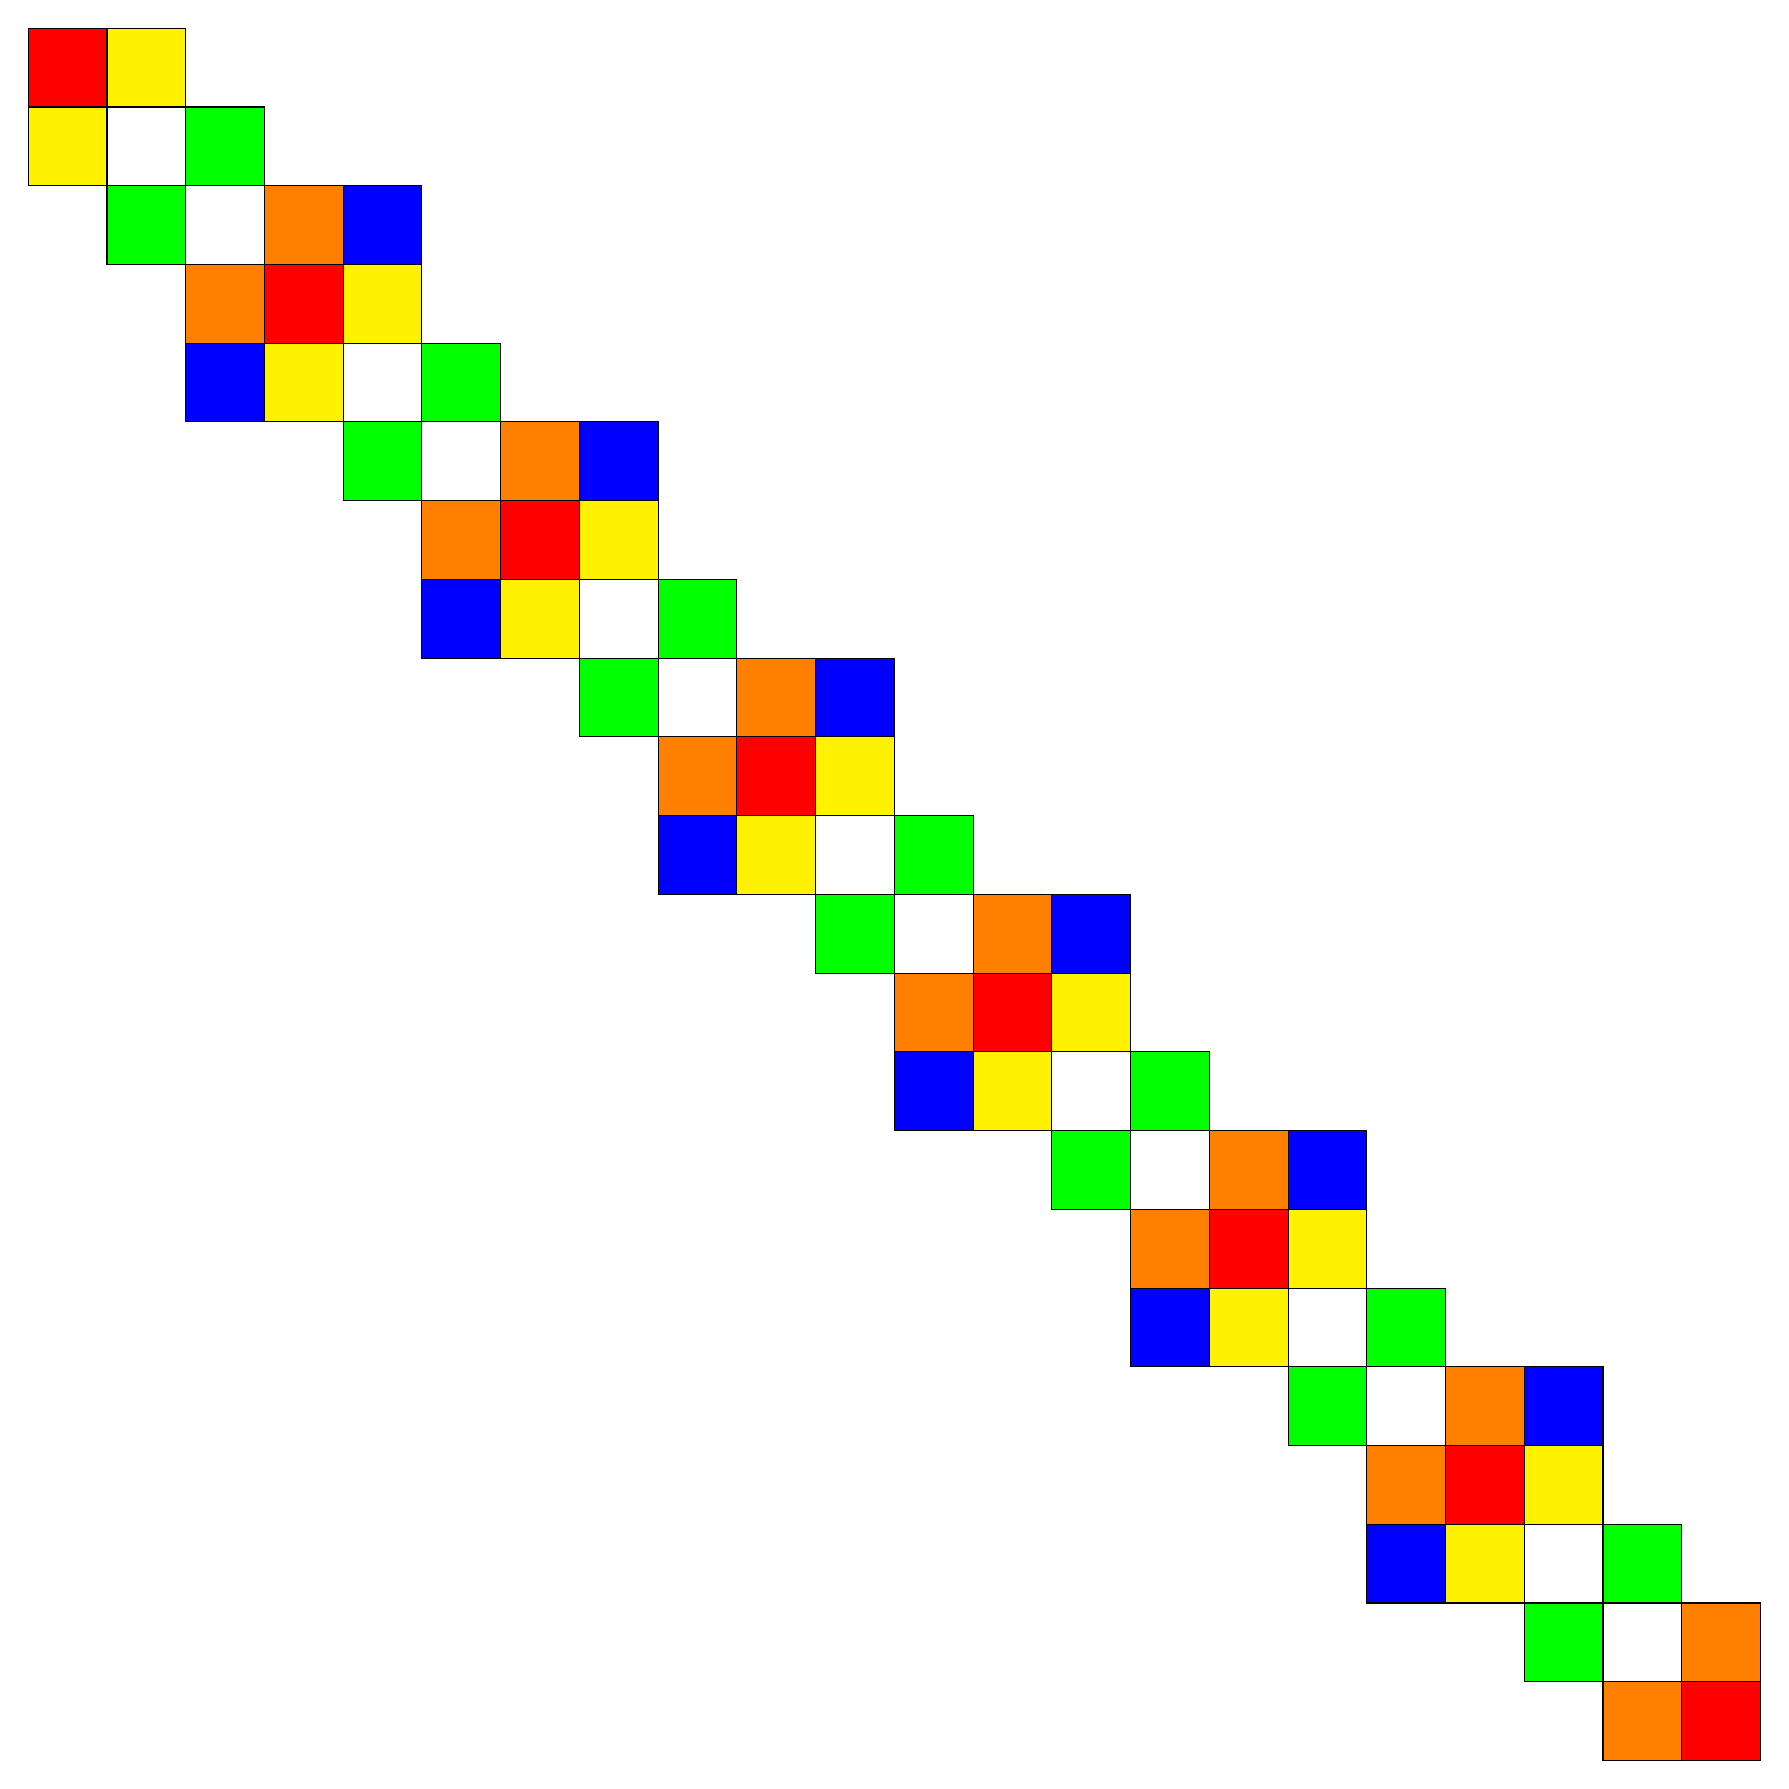
\begin{tikzpicture}
\foreach \i in {0,...,7} {
	\draw [fill=red](3*\i,-3*\i) rectangle (3*\i+1,-3*\i-1);
}
\foreach \i in {0,...,6} {
	\draw [fill=yellow](3*\i+1,-3*\i) rectangle (3*\i+2,-3*\i-1);
	\draw [fill=yellow](3*\i,-3*\i-1) rectangle (3*\i+1,-3*\i-2);
	\draw [fill=green](3*\i+2,-3*\i-1) rectangle (3*\i+3,-3*\i-2);
	\draw [fill=green](3*\i+1,-3*\i-2) rectangle (3*\i+2,-3*\i-3);
	\draw [fill=orange](3*\i+3,-3*\i-2) rectangle (3*\i+4,-3*\i-3);
	\draw [fill=orange](3*\i+2,-3*\i-3) rectangle (3*\i+3,-3*\i-4);
}
\foreach \i in {0,...,5} {
	\draw [fill=blue](3*\i+4,-3*\i-2) rectangle (3*\i+5,-3*\i-3);
	\draw [fill=blue](3*\i+2,-3*\i-4) rectangle (3*\i+3,-3*\i-5);
}
\end{tikzpicture}
\end{document}
